
%(BEGIN_QUESTION)
% Copyright 2013, Tony R. Kuphaldt, released under the Creative Commons Attribution License (v 1.0)
% This means you may do almost anything with this work of mine, so long as you give me proper credit

This level control system has a problem.  The liquid level has fallen below setpoint and is continuing to decrease over time, as indicated both by the controller and the sightglass.  The controller's display also shows the output signal to be -1\%:

$$\includegraphics[width=15.5cm]{i03387x01.eps}$$

Identify the likelihood of each specified fault for this circuit.  Consider each fault one at a time (i.e. no coincidental faults), determining whether or not each fault could independently account for {\it all} measurements and symptoms in this circuit.

% No blank lines allowed between lines of an \halign structure!
% I use comments (%) instead, so that TeX doesn't choke.

$$\vbox{\offinterlineskip
\halign{\strut
\vrule \quad\hfil # \ \hfil & 
\vrule \quad\hfil # \ \hfil & 
\vrule \quad\hfil # \ \hfil \vrule \cr
\noalign{\hrule}
%
% First row
{\bf Fault} & {\bf Possible} & {\bf Impossible} \cr
%
\noalign{\hrule}
%
% Another row
250 ohm resistor failed open &  &  \cr
%
\noalign{\hrule}
%
% Another row
I/P transducer coil failed open &  &  \cr
%
\noalign{\hrule}
%
% Another row
I/P transducer nozzle plugged &  &  \cr
%
\noalign{\hrule}
%
% Another row
Wire open between TB4 and level transmitter &  &  \cr
%
\noalign{\hrule}
%
% Another row
Wire open between TB5 and I/P transducer &  &  \cr
%
\noalign{\hrule}
%
% Another row
Manual bypass valve open too far &  &  \cr
%
\noalign{\hrule}
%
% Another row
Circuit breaker \#15 tripped (off) &  &  \cr
%
\noalign{\hrule}
} % End of \halign 
}$$ % End of \vbox

\underbar{file i03387}
%(END_QUESTION)





%(BEGIN_ANSWER)

% No blank lines allowed between lines of an \halign structure!
% I use comments (%) instead, so that TeX doesn't choke.

$$\vbox{\offinterlineskip
\halign{\strut
\vrule \quad\hfil # \ \hfil & 
\vrule \quad\hfil # \ \hfil & 
\vrule \quad\hfil # \ \hfil \vrule \cr
\noalign{\hrule}
%
% First row
{\bf Fault} & {\bf Possible} & {\bf Impossible} \cr
%
\noalign{\hrule}
%
% Another row
250 ohm resistor failed open &  & $\surd$ \cr
%
\noalign{\hrule}
%
% Another row
I/P transducer coil failed open &  & $\surd$ \cr
%
\noalign{\hrule}
%
% Another row
I/P transducer nozzle plugged & $\surd$ &  \cr
%
\noalign{\hrule}
%
% Another row
Wire open between TB4 and level transmitter &  & $\surd$ \cr
%
\noalign{\hrule}
%
% Another row
Wire open between TB5 and I/P transducer &  & $\surd$ \cr
%
\noalign{\hrule}
%
% Another row
Manual bypass valve open too far & $\surd$ &  \cr
%
\noalign{\hrule}
%
% Another row
Circuit breaker \#15 tripped (off) &  & $\surd$ \cr
%
\noalign{\hrule}
} % End of \halign 
}$$ % End of \vbox

%(END_ANSWER)





%(BEGIN_NOTES)

{\bf This question is intended for exams only and not worksheets!}.

%(END_NOTES)


